\documentclass{beamer}

\usepackage[utf8x]{inputenc}
\usepackage{graphicx}
\usepackage{tabularx}
\usepackage{listings}
\usepackage[brazil]{babel}
\usetheme{Luebeck}
%\usetheme{Singapore}
\usecolortheme{rose}

\title[Operações Geométricas (Warping) em Imagens]{Operações Geométricas
(Warping) em Imagens}
\author[Roberto Azevedo]{Roberto Gerson de Albuquerque Azevedo}
\institute{Foundations of Computer Graphics 2011.1 PUC-Rio}
\date{\today}
\subject{alguma coisa}
%\logo{\includegraphics[scale=1.0]{sua_figura.png}}

\lstset{language=C}

\begin{document}
%para criar a página de rosto
\frame{\titlepage} %inclui a front page 
%==================================================slide
% cria o sumário
\begin{frame}
 \frametitle{Sumário}
 \tableofcontents
\end{frame}
%-------------------------------------------------------
%==================================================slide
\section{Introdução}
\begin{frame}
\frametitle{Introdução}
\begin{itemize}
 \item Operações Geométricas (ou filtros geométricos, ou \textit{Warping}) tem
como objetivo alterar as posições dos pixels da imagem, baseada em alguma função
de mapeamento.
  \item Extremamente útil para o mapeamento de texturas.
  \item Em princípio, uma operação geométrica transforma uma dada imagem $I$
para uma nova imagem $I'$ modificando as coordenadas dos pixels da imagem:
\par
\begin{center}
 $I(x,y) \rightarrow I'(x', y')$
\end{center}

\end{itemize}
\end{frame}

%-------------------------------------------------------
%==================================================slide
\subsection{Exemplos}
\begin{frame}
 \frametitle{Transformações Geométricas - Exemplos}
\begin{figure}[ht!]
  \centering
  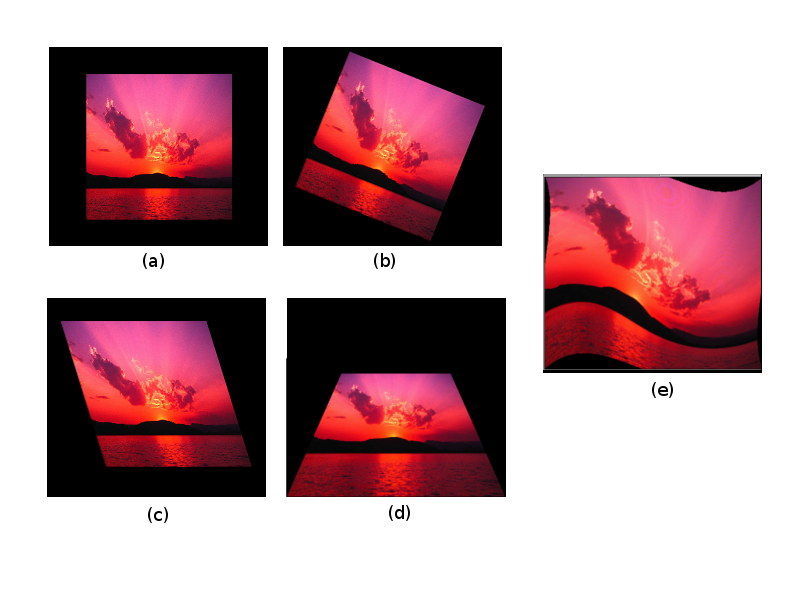
\includegraphics[width=0.70\textwidth]{img/typical-geometric-transform.png}
\end{figure}
Exemplos de transformações geométricas em imagens: (a) escala; (b) rotação; (c)
cisalhamento; (d) perpectiva; e (e) twirl.
\end{frame}

%-------------------------------------------------------
%==================================================slide
\subsection{Reamostragem e Interpolação}
\begin{frame}
\frametitle{Transformações Geométricas - Problemas}
\begin{itemize}
 \item Operações geométricas não são simples, porque envolvem reamostrar os
pixels que inicialmente são discretos em um domínio de reais.
 \item Problemas:
 \begin{itemize}
  \item Magnificação - duplica informação (serrilhado)
  \item Minimificação - perde informação (\textit{aliasing})
 \end{itemize}
\end{itemize}
\begin{figure}[ht!]
  \centering
  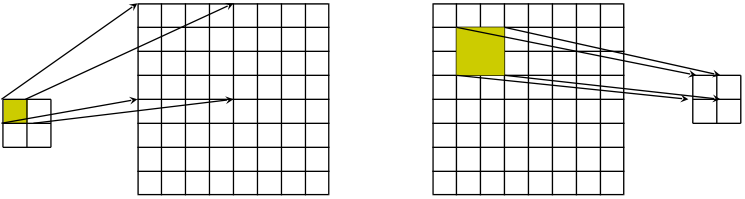
\includegraphics[width=0.8\textwidth]{img/resize.png}
\end{figure}
\end{frame}

%-------------------------------------------------------
%==================================================slide
\begin{frame}
  \frametitle{Reamostragem: Interpolação}
\begin{itemize}
 \item A função de mapeamento comumente é uma função $R^2 \rightarrow R^2$.
 \item Como tanto a imagem original como a imagem final são discretas, quase
sempre temos um problema de reamostragem depois de aplicar a função de
mapeamento.
\end{itemize}
\pause
\begin{center}
 \framebox{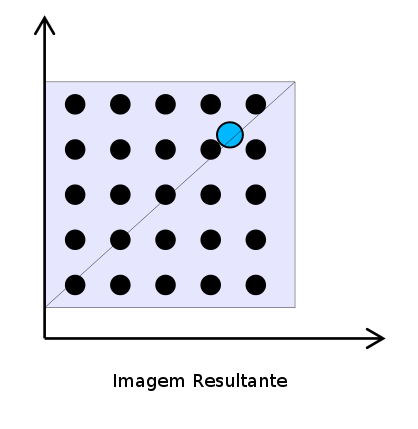
\includegraphics[width=1.2in]{img/pixels-in-resulting-image.png}}
\end{center}
\end{frame}

%-------------------------------------------------------
%==================================================slide
\begin{frame}
  \frametitle{Reamostragem: "Interpolação" (Nearest Neighbor)}
\begin{itemize}
 \item Escolhe o pixel mais próximo do qual ele deveria ser mapeado.
\end{itemize}
\begin{center}
 \framebox{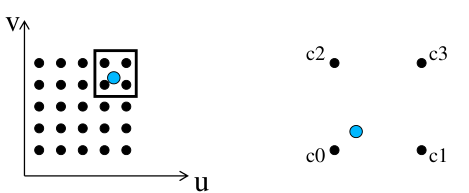
\includegraphics[width=2.5in]{img/nearest-neighbor.png}}
\end{center}
\pause
  $x = (int) floatx + 0.5;$ \\
  $y = (int) floatx + 0.5;$
\end{frame}

%-------------------------------------------------------
%==================================================slide
\begin{frame}[fragile]
  \frametitle{Reamostragem: Interpolação Bilinear}
\begin{itemize}
 \item Escolhe a cor a partir da composição de 3 interpolações.\\
\end{itemize}
\begin{center}
 \framebox{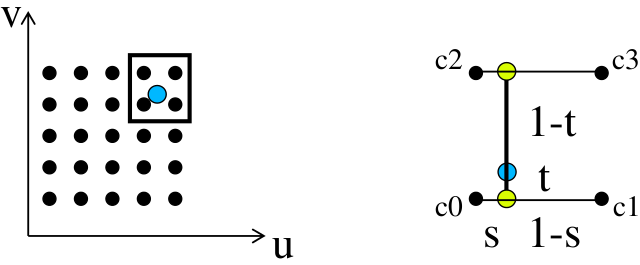
\includegraphics[width=2.5in]{img/bilinear-interpolation.png}}
\end{center}
\pause
\tiny
\begin{lstlisting}
void imgBillinearInterpolate(float xW, float yW, float* nw,
        float *ne, float *sw, float *se, float *result)
{
  float cx = 1.0f - xW;
  float cy = 1.0f - yW;

  float m0, m1;
  /* red */
  m0 = cx*nw[0] + xW*ne[0];
  m1 = cx*sw[0] + xW*se[0];
  result[0] = (cy*m0 + yW*m1);
  ...
}
\end{lstlisting}
\end{frame}

%-------------------------------------------------------
%==================================================slide
\subsection{Classificação}
\begin{frame}
 \frametitle{Transformações Geométricas - Classificação}
\begin{figure}[ht!]
  \centering
  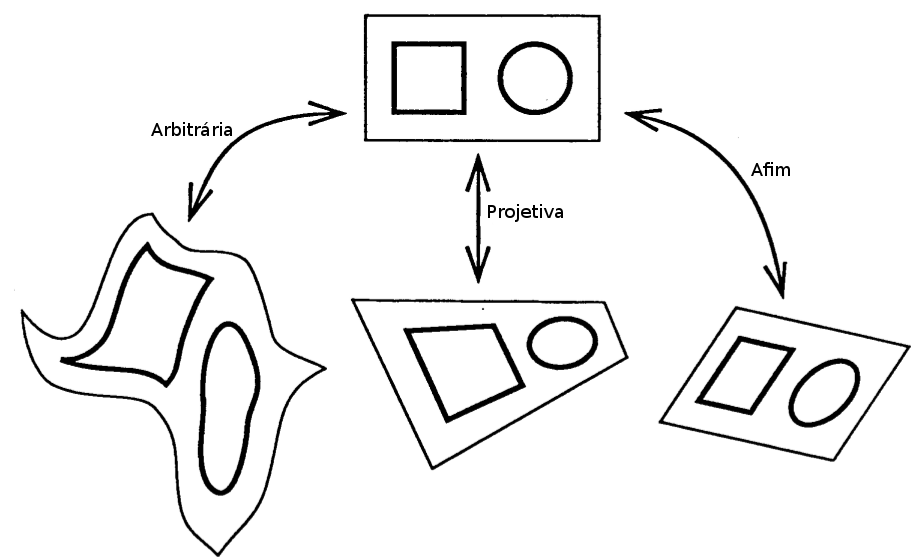
\includegraphics[width=0.75\textwidth]{img/affine-projective-arbitrary.png}
\end{figure}
\end{frame}

%-------------------------------------------------------
%==================================================slide
\section{Funções de Mapeamento}
\begin{frame}
\frametitle{Reamostragem: Source-to-target X Target-to-source}
\begin{tabular*}{0.75\textwidth}{ p{4cm} p{.6cm} p{4cm}}
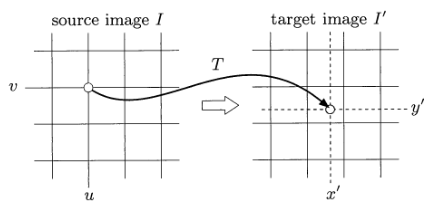
\includegraphics[width=1.9in]{img/source-to-target-mapping.png}  & &
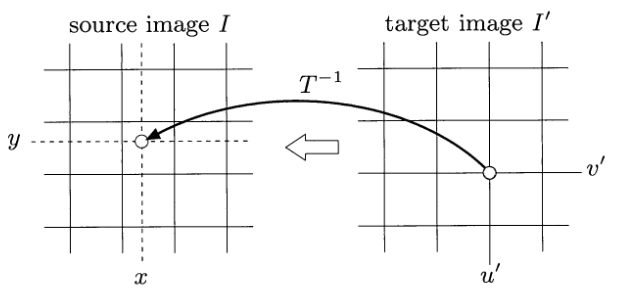
\includegraphics[width=1.9in]{img/target-to-source-mapping.png} \\
\scriptsize
\textbf{Source-to-target}: Para cada pixel $(x,y)$ da imagem original
$I$ a posição transformada em $I'$ é dada por: 
\begin{equation*}
 (u,v)=T(x,y)
\end{equation*} & &
\scriptsize
\textbf{Target-to-source}: Para cada pixel $(u',v')$ da imagem final
$I'$, é computado o ponto correspondente (contínuo) da imagem original: 
\begin{equation*}
 (x, y)=T^{-1}(u',v')
\end{equation*} \\
\end{tabular*}
\end{frame}

%-------------------------------------------------------
%==================================================slide
\subsection{Twirl}
\begin{frame}
\frametitle{Twirl}
\begin{itemize}
 \item A transformação "Twirl" faz uma rotação na imagem ao redor de um dado
ponto $p_c = (x_c, y_c)$ com variação espacial em relação ao ângulo de rotação
$\alpha$.
 \item A imagem se mantém inalterada fora de um limite dado por $r_{max}$.
\end{itemize}

\begin{columns}[c]
\column{1.5in}
\textbf{Input:} \\
Centro: $p_c = (x_c, y_c)$ \\
Ângulo de Rotação: $\alpha$ \\
Raio Máximo: $r_{max}$ 
\column{1.5in}
\framebox{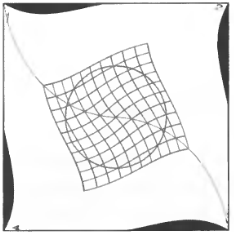
\includegraphics[width=1.5in]{img/twirl.png}}
\end{columns}
\end{frame}

%-------------------------------------------------------
%==================================================slide
\begin{frame}
\frametitle{Twirl: Função de Mapeamento Inverso}
A Função de Mapeamento inverso da transformação \textit{twirl} (dado um ponto da
textura $(u,v)$, determina o ponto correspondente na image) é dada por:
   \begin{equation}
    T_x^{-1}: x = 
\begin{cases}
 x_c + r.cos(\beta), & \text{se } r \leq r_{max}\\
 x', & \text{se } r > r_{max}
\end{cases}
   \end{equation}

\begin{equation}
    T_y^{-1}: y = 
\begin{cases}
 y_c + r.sin(\beta), & \text{se } r \leq r_{max} \\
 y', & \text{se } r > r_{max}
\end{cases}
\end{equation}

\pause
Onde,
\begin{equation}
\begin{array}{c|c}
d_x = x'- x_c & r = \sqrt[2]{d_x^2+d_y^2} \\
d_y =  y'- y_c & \beta = AcTang(s_x, d_y + \alpha.(\frac{r_max-r}{r_max}))
\end{array}
\end{equation}
\end{frame}

%-------------------------------------------------------
%==================================================slide
\subsection{Spherical}
\begin{frame}
 \frametitle{Spherical}
\begin{itemize}
 \item A deformação esférica imita o efeito de visualizar uma imagem por meio
de uma meia esfera ou lente posta sobre a imagem.
\end{itemize}
 
\begin{columns}[c]
\column{1.5in}
\textbf{Input:} \\
Centro da lente esférica: $p_c = (x_c, y_c)$
Raio da lente: $r_{max}$
Índice de refração: $\rho$
\column{1.5in}
\framebox{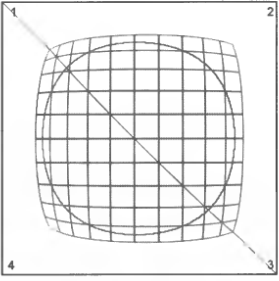
\includegraphics[width=1.5in]{img/sphere.png}}
\end{columns}
\end{frame}

\begin{frame}
 \frametitle{Spherical: Função de mapeamento inverso.}
  \begin{equation}
    T_x^{-1}: x = x' -
\begin{cases}
 z.tan(\beta_x), & \text{se }\;\; r \leq r_{max}\\
 0, & \text{se }\;\; r > r_{max}
\end{cases}
   \end{equation}

\begin{equation}
    T_y^{-1}: y = y' - 
\begin{cases}
 z.tan(\beta_y), & \text{se } r \leq r_{max} \\
 0, & \text{se } r > r_{max}
\end{cases}
\end{equation}

Onde,
\begin{equation}
\begin{array}{c|c|c}
d_x = x'- x_c & r = \sqrt[2]{d_x^2+d_y^2}  & \beta_x =
(1-\frac{1}{\rho}.sin^-1(\frac{d_x}{\sqrt[2]{d_x^2+z^2}}))\\
 & & \\
d_y =  y'- y_c & z = \sqrt[2]{r_max^2 - r^2} & \beta_y = 
(1-\frac{1}{\rho}.sin^-1(\frac{d_x}{\sqrt[2]{d_y^2+z^2}}))
\end{array}
\end{equation}
\end{frame}

%-------------------------------------------------------
%==================================================slide
\subsection{Projeção perspectiva}
\begin{frame}
 \frametitle{Projeção Perspectiva}
 \begin{itemize}
  \item A projeção perspectiva é uma transformação linear entre quadriláteros
arbitrários.
  \item Uma projeção perspectiva é uma (caso especial de) Homografia!
  \item Algumas propriedades:
  \begin{itemize}
   \item Todas as linhas continuam sendo linhas.
   \item Uma composição de duas perspectivas não é uma perspectiva.
  \end{itemize}
 \end{itemize}
\begin{center}
\framebox{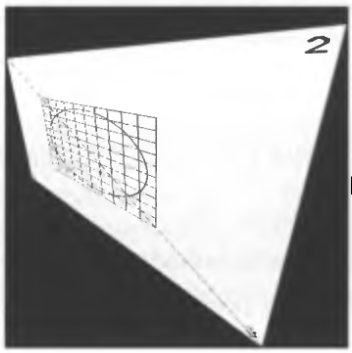
\includegraphics[width=1.5in]{img/perspective.png}}
\end{center}
\end{frame}

%-------------------------------------------------------
%==================================================slide
\begin{frame}
\frametitle{Projeções perspectivas}

\[
 \begin{bmatrix}
      uq & vq & q
  \end{bmatrix} 
  = 
  \begin{bmatrix} x & y & 1 \end{bmatrix} . 
\begin{bmatrix} 
a & d & g \\
b & e & h \\
c & f & i \\  
\end{bmatrix}
\]

Onde pode-se tirar que: \\
\begin{columns}[c]
\column{2.0in}
$u = \frac{ax + by + c}{gx + hy + i}$
\column{2.0in}
$v = \frac{dx + ey + f}{gx + hy + i}$
\end{columns}
\end{frame}

%-------------------------------------------------------
%==================================================slide
\begin{frame}
\frametitle{Composição de Projeção perspectiva}
\begin{center}
\framebox{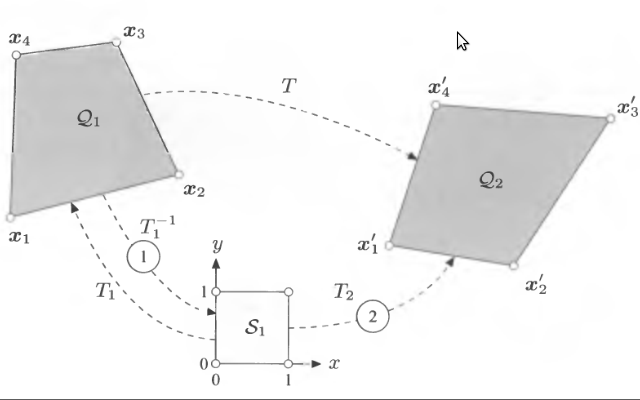
\includegraphics[width=3.0in]{img/two-step-projective-transform.png}}
\end{center}
\end{frame}

%-------------------------------------------------------
%==================================================slide
\section{EWA - Elliptical Weighted Average Filter}
\begin{frame}
\frametitle{Filtro EWA}
 \begin{itemize}
  \item EWA: Elliptical Weighted Average Filter.
  \item Compensa artefatos de \textit{aliasing} causados pela projeção
perspectiva.
 \end{itemize}
\end{frame}

\begin{frame}[fragile]
\frametitle{EWA - Algoritmo}
O Algoritmo é dado pelos passos a seguir:
\begin{itemize}
 \item Cálculo da Homografia.
 \item Cálculo dos pesos.
 \item Para cada pixel da imagem resultante:
 \begin{itemize}
  \item Cálculo da Matriz Jacobiana (Aproximação de uma transformação afim
naquele ponto)
  \item Cálculo dos Coeficientes da Elipse.
  \item Cálculo do centro da Elipse.
  \item Aplica o filtro EWA naquele pixel.
 \end{itemize}
\end{itemize}
\end{frame}

%-------------------------------------------------------
%==================================================slide
\begin{frame}[fragile]
 \frametitle{EWA - Código}
\tiny
\begin{lstlisting}
m3Homography4p (pu, pv, px, py, Hom);
m3Inv(Hom, HomInv);
ewaWeigths(wtab, EWA_WTAB_SIZE, EWA_ALPHA);

for(y=0; y<h; y++)
{
  for(x=0; x<w; x++)
  {
    ewaJacobianCoefficients(x, y, HomInv, &Ux, &Uy, &Vx, &Vy);
    ewaEllipseCoefficients(Ux, Uy, Vx, Vy, &A, &B, &C, &F, EWA_ENHANCED);
    ewaEllipseCenter(x, y, HomInv, &U0, &V0);

    ewaFilter(img, U0, V0, wtab, A, B, C, F, rgb);
    imgSetPixel3fv(img1, x, y, rgb);
  }
}
\end{lstlisting}
\end{frame}

%-------------------------------------------------------
%==================================================slide
\begin{frame}[fragile]
 \frametitle{EWA - Passos}
1. Cálculo dos Pesos:
\tiny
\begin{lstlisting}
void ewaWeigths(double *weigths, int length, double alpha)
{
  double r;
  int i;
  for(int i = 0; i < length; i++)
  {
    r = i/(double) (length - 1);
    weigths[ i ] = exp( - alpha * r);
  }
}
\end{lstlisting}

\pause
\small
2. Cálculo da Jacobiana:
\[
J=\left[ \begin{array}{cc}
\frac{\partial u}{\partial x} & \frac{\partial u}{\partial y} \\
\frac{\partial v}{\partial x} & \frac{\partial v}{\partial y} 
\end{array}
\right]
= 
\left[ \begin{array}{cc}
U_x & U_y \\
V_x & V_y 
\end{array}
\right]
\]
\end{frame}

%-------------------------------------------------------
%==================================================slide

\begin{frame}[fragile]
\frametitle{EWA - Passos}
3. Coeficientes da Elipse: \\
\begin{columns}[c]
\column{2.0in}
\textit{EWA Normal}:
$A = Vx.Vx + Vy.Vy$ \\
$B = (-2).(Ux.Vx + Uy.Vy)$ \\
$C = Ux.Ux + Uy.Uy$
$F = (Ux.Vy - Uy.Vx)^2$
\column{2.0in}
\textit{Enhanced EWA}
$A = Vx.Vx + Vy.Vy + 1$
$B = -2.(Ux.Vx + Uy.Vy)$
$C = Ux.Ux + Uy.Uy + 1$
$F = A.C - \frac{(B.B)^2}{4}$
\end{columns}
\end{frame}

%-------------------------------------------------------
%==================================================slide
\begin{frame}
\frametitle{Conclusões}
\begin{itemize}
 \item Transformações geométricas não são trivias, principalmente porque
envolve reamostragem dos pixels em um domínio contínuo.
 \item Reamostragem possivelmente causa problemas de \textit{aliasing}.
 \item O filtro EWA é uma solução que busca diminuir esse problema.
 \item Possíveis Trabalhos Futuros
 \begin{itemize}
  \item Outras transformações geométricas.
  \item Outras interpolações (Trilinear, B-spline etc.)
  \item Morphing.
  \item Testar outros pré-filtros que não o gaussiano para o EWA.
 \end{itemize}
\end{itemize}
\end{frame}

%-------------------------------------------------------
%==================================================slide
\begin{thebibliography}{10}
\bibitem{Crane1997}[Crane, 1997]
Randy Crane.
\newblock A simplified Approach to Image Processing: Classical and Modern
Techniques in C.

\bibitem{Burger1997}[Burger and Burge, 2008]
Wilhelm Burger and Mark J. Burge
\newblock Digital Imaging Processing: An algorithm introduction using Java.

\bibitem{Herckbert1989}[Herckbert, 1989]
Paul S. Heckbert
\newblock Fundamentals of Texture Mapping and Image Warping.

\bibitem{Slusallek}[Slusallek, ????]
Philipp Slusallek
\newblock Computer Graphics: Texture Filtering and Spectral Analysis
(Presentation).
\end{thebibliography}

\end{document}
